\documentclass[letterpaper, 10 pt, conference]{ieeeconf}  % Comment this line out if you need a4paper
%\documentclass[a4paper, 10pt, conference]{ieeeconf}   % Use this line for a4 paper
\IEEEoverridecommandlockouts                                    % This command is only needed if you want to use the \thanks command
\overrideIEEEmargins                                                 % Needed to meet printer requirements.

%In case you encounter the following error:
%Error 1010 The PDF file may be corrupt (unable to open PDF file) OR
%Error 1000 An error occurred while parsing a contents stream. Unable to analyze the PDF file.
%This is a known problem with pdfLaTeX conversion filter. The file cannot be opened with acrobat reader
%Please use one of the alternatives below to circumvent this error by uncommenting one or the other
%\pdfobjcompresslevel=0
%\pdfminorversion=4

% See the \addtolength command later in the file to balance the column lengths
% on the last page of the document

\usepackage{graphicx}    % for pdf, bitmapped graphics files
%\usepackage{epsfig}    % for postscript graphics files
\usepackage{mathptmx} % assumes new font selection scheme installed
\usepackage{times}        % assumes new font selection scheme installed
\usepackage{amsmath}  % assumes amsmath package installed
\usepackage{amssymb}  % assumes amsmath package installed
\usepackage{listings}

\title{\LARGE \bf Formation Control}

\author{Ajay Ahir, Ben Philps and Sumaiyah Kola}

\begin{document}

\maketitle
\thispagestyle{empty}
\pagestyle{empty}

%%%%%%%%%%%%%%%%%%%%%%%%%%%%%%%%%%%%%%%%%%%%%%%%%%%%%%%%%%%%%%%%%%%%%%%%%%%%%%%%
\begin{abstract}

Multi-robot teams may need to move in formation for various reasons such as surveillance or purely for display. This report describes a project undertaken to perform the navigation of multi-robot teams with formation control using a behavior based approach. These behaviors generate velocities that combine to lead each robot, such as by generating a velocity to avoid obstacles and a velocity to remain in formation. Both a centralized and decentralized solution are shown.

\end{abstract}

%%%%%%%%%%%%%%%%%%%%%%%%%%%%%%%%%%%%%%%%%%%%%%%%%%%%%%%%%%%%%%%%%%%%%%%%%%%%%%%%
\section{INTRODUCTION}
\label{introductionsection}

Robots that are part of a multi-robot team may need to navigate an environment in formation, perhaps as part of a display or to guarantee 360$^{\circ}$ coverage during surveillance. However, staying in formation while navigating may not be possible. Take tight corridors for example - a wide diamond formation may not fit, thus preventing the robots from fulfilling their purpose and leading to a state where they are stuck. The problem here is finding a way to split and merge the robots, so that they can navigate around obstacles and through limited space by momentarily breaking formation before getting back into formation. \\

In order to solve this problem, we use the approach taken in this$^{\cite{behaviorpaper}}$ paper which defines behaviors for each robot. These behaviors break down the task of formation control into behavioral components, and these are: formation maintenance, goal navigation, and static/dynamic obstacle avoidance. Each behavior generates a velocity, also called a `motor schema', and these are summed to generate the overall motion of each robot. By weighting each component velocity differently in the sum, the behavior of the resulting motion can be altered, and this is detailed under \ref{combiningsubsection}. \\

Both a centralized and decentralized solution are viable options, as any practical scenario may not have guaranteed centralized communication, so both approaches are considered and shown. Where the centralized solution uses the knowledge of all robots positions and their combined view of the world, the decentralized solution shows how this can be achieved by each individual robot and using limited message passing. \\

Our setup uses ROS$^{\cite{ros}}$ to control our robots, which are standard Turtlebot3's$^{\cite{turtlebot}}$. We use Gazebo$^{\cite{gazebo}}$ as our simulation environment. With these tools we can launch multiple robots into a world which run our algorithms. These worlds are created by defining the objects within the world using `world' files which Gazebo understands. Fig. \ref{corridorworld} shows such an example world.

\begin{figure}[thpb]
\centering
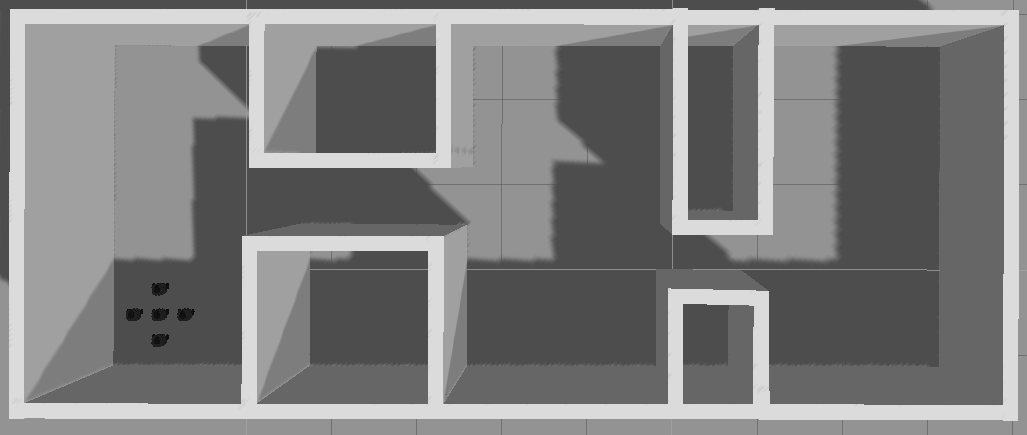
\includegraphics[width=\linewidth]{corridorworld}
\caption{Example world in Gazebo}
\label{corridorworld}
\end{figure}

With this setup we begin our implementation.

\section{APPROACH}

\subsection{Formations}
\label{formationsubsection}

For our solution$^{\cite{repository}}$, we first define the formations we use. Each formation is given by a vector of relative $(x,y)$ coordinates for $5$ robots, where the point $(0,0)$ is the center of the formation. Each robot has an ID which indexes this vector to determine its relative position. Our formations are: \\

\begin{itemize}
\item \textbf{Line} - $[(0.6,0), (0.3,0), (0,0), (\text{-}0.3,0), (\text{-}0.6,0)]$
\item \textbf{Column} - $[(0,0.6), (0,0.3), (0,0), (0,\text{-}0.3), (0,\text{-}0.6)]$
\item \textbf{Diamond} - $[(0,0), (\text{-}0.3,\text{-}0.3), (0,\text{-}0.3), (0,\text{-}0.6), (0.3,\text{-}0.3)]$
\item \textbf{Wedge} - $[(0.6,\text{-}0.3), (0.3,0), (0,0), (\text{-}0.3,0), (\text{-}0.6,\text{-}0.3)]$
\end{itemize}~

The $0.3$ spacing distance between each robot is controlled by a variable which adjusts the compactness of the formation. In the centralized solution all robot positions are known, and more importantly the formation origin is known so each robot's relative position can be computed. In the decentralized solution this information is unknown and has to be communicated. Each formation thus defines `links' between robots that are able to communicate based on where they are in the formation. In line, column, and wedge the robots can communicate with the robots directly next to each other i.e. the adjacent relative position. In diamond, the robots are arranged such that they can all communicate with the central robot in relative position $(0,\text{-}0.3)$.

Having these formations ready we move on to generating each of the behaviors that define our motion.

\subsection{Formation Velocity}

Two methods for keeping the robots in formation were considered. The first is called Unit Reference, where the average position taken across all robots is used to define the point around which the formation is held. Each robot then generates a velocity to an offset from this position, which defines their place in the formation, as given by a robot ID preassigned to them. Whilst this solution is straightforward to implement in a centralized fashion, its disadvantage is that in a decentralized implementation every robot is required to know the position of every other robot in order to find the formation center. \\

TODO: do we want equations here that show how to generate robot positions using averages+offset? \\

The approach we took is called Leader-Follower. With this approach a certain robot is designated the leader, which is chosen based on their ID and whichever one corresponds to the $(0,0)$ offset. The leader does not need to calculate a formation velocity, as it is always considered to be in formation. The other `follower' robots then use the leader's position to generate the velocity to their position. \\

TODO: add explanation and pseudocode for get\_desired\_position \\

The direction is easily calculated by subtraction of position vectors. This vector is normalized after calculating its magnitude, which is the distance from the robot to the target position. The final speed is determined by this distance and where it lies within two `zones'. These zones are called the `dead zone' and `control zone'. The dead zone is a small region around the goal at which the velocity is considered zero, which deals with positional noise and error when moving to the target position. Inside the control zone the velocity is scaled proportional to this distance to control speed, and outside the control zone the velocity is capped to what it would be if it were on the edge of the control zone. Fig. \ref{zonecode} shows this in pseudocode.

\begin{figure}[thpb]
\centering
\lstset{language=python}
\begin{lstlisting}
if distance < DEAD_ZONE:
  velocity = velocity * 0.
else if distance < CONTROL_ZONE:
  velocity = velocity * distance
else
  velocity = velocity * CONTROL_ZONE
\end{lstlisting}
\caption{Formation velocity pseudocode}
\label{zonecode}
\end{figure}

Our value for the dead zone is $1.5$ times the robot radius, which comes to $0.07875$. The control zone is defined as the dead zone plus the formation spacing distance described in \ref{formationsubsection}.

Decentralizing the Leader-Follower solution is a much easier task, as only the leader robot's position is required. Each robot then participates in message passing to get the position from the leader, and uses this to execute exactly the same code.

\subsection{Goal Velocity}

With the Leader-Follower approach to formation control, only the leader needs a goal velocity as the followers' goal is defined by their position in the formation, and this velocity component comes from the Formation Velocity behavior. Our leader runs the RRT* algorithm once to compute an obstacle free path to a goal. \\

TODO: brief explanation of RRT* and how the vector to the path is generated \\

This solution naturally extends to being decentralized, as it is only executed for one robot in the centralized case, and therefore only the leader needs to execute it in the decentralized case. A robot knows they are the leader when their offset in the formation is $(0,0)$.

\subsection{Static/Dynamic Obstacle Avoidance Velocity}

TODO: update this first paragraph with details on the leader's obstacle avoidance \\

Our implementation of RRT* has built-in obstacle avoidance, so the leader does not need to compute a velocity vector for static obstacles. Each follower robot however uses laser sensors to obtain measurements that determine its distance to obstacles within a 180$^{\circ}$ cone in front of it. These measurements are fed into a rule based obstacle avoidance controller which steers the robot away from static obstacles such as walls. \\

TODO: need to determine the level of detail or if any pseudocode is provided for this

TODO: update the following paragraph with details of new robot avoidance \\

The dynamic obstacles are other robots, and the laser sensors are quite poor at detecting other robots which is why a separate implementation is required. Our implementation of this uses the position of each robot to produce a weight vector instead of a velocity vector. This weight acts as an `on-off' switch which stops a robot from moving if it is too close to another robot, and thus takes the value $0$ or $1$. We stop the robot with the lowest ID, as this reduces the combinatorial complexity to $O(n^{2})$ as we only need to consider each possible pair of robots. While there are edge cases to this approach, the weak sensor measurements should still activate the obstacle avoidance to allow the robot that is not left stationary to move. \\

One downside to this however is that decentralizing this method cannot currently be achieved, as each robot in the decentralized implementation only maintains a belief of the leader's position, and not any other robot. Therefore there is more dependence on the sensors and the obstacle avoidance's robustness.

\subsection{Combining Velocities}
\label{combiningsubsection}

TODO: check the weights in here match the final version of the code \\

Each velocity component is combined with a weight. This weight affects the nature of the robots movement. The weights we used were $0.8$ for the goal velocity, $1.2$ for the formation velocity, and $3.0$ for the static obstacle avoidance velocity. The resulting behavior forces the robots to stay in formation when there is free space, with the added effect of the followers playing `catch-up' with the leader to avoid being left behind. In the presence of obstacles, the robots will split to avoid the obstacles and merge once they are free again.

The vector of dynamic obstacle avoidance weights will stop robots that get too close from moving, and the robots also stop moving once they are at their goal to avoid other velocity components from leading to erroneous and spurious movements. \\

TODO: perhaps some pseudocode

TODO: need to add that these are [x,y] velocities later turned into [u,w]

\subsection{Centralized and Decentralized solution}

The centralized solution uses the algorithms defined above and the known position of each robot, called the `ground truth', to compute their velocity vectors. This is achieved with the setup described in \ref{introductionsection}. \\

The decentralized solution uses the modified versions of the algorithms also defined above and message passing to learn the leader robot's position. The setup required is slightly different. Whilst we still launch a single world, a copy of the robot code must be launched for each robot. \\

We now look at the results from our implementations.

\section{RESULTS}

TODO - show maps, image traces of simulations, talk about accuracy, robustness, efficiency

\section{CONCLUSION}

TODO - success, robustness (completeness), future work (i.e. improving decentralized)

\subsection{Figures and Tables}

Positioning Figures and Tables: Place figures and tables at the top and bottom of columns. Avoid placing them in the middle of columns. Large figures and tables may span across both columns. Figure captions should be below the figures; table heads should appear above the tables. Insert figures and tables after they are cited in the text. Use the abbreviation Fig. 1, even at the beginning of a sentence.

\begin{table}[h]
\caption{An Example of a Table}
\label{table_example}
\begin{center}
\begin{tabular}{|c||c|}
\hline
One & Two\\
\hline
Three & Four\\
\hline
\end{tabular}
\end{center}
\end{table}

\addtolength{\textheight}{-12cm}   % This command serves to balance the column lengths
                                               % on the last page of the document manually. It shortens
                                               % the textheight of the last page by a suitable amount.
                                               % This command does not take effect until the next page
                                               % so it should come on the page before the last. Make
                                               % sure that you do not shorten the textheight too much.

%%%%%%%%%%%%%%%%%%%%%%%%%%%%%%%%%%%%%%%%%%%%%%%%%%%%%%%%%%%%%%%%%%%%%%%%%%%%%%%%

\section{ACKNOWLEDGMENT}

\begin{itemize}
\item Ajay Ahir - 
\item Ben Philps - 
\item Sumaiyah Kola - 
\end{itemize}

%%%%%%%%%%%%%%%%%%%%%%%%%%%%%%%%%%%%%%%%%%%%%%%%%%%%%%%%%%%%%%%%%%%%%%%%%%%%%%%%

\begin{thebibliography}{99}

\bibitem{behaviorpaper} T. Balch and R. C. Arkin. Behavior-based Formation Control for Multi-robot Teams. IEEE Transactions on Robotics and Automation, 1999.
\bibitem{ros} ROS - Robot Operating System. https://www.ros.org/
\bibitem{turtlebot} Turtlebot3. http://emanual.robotis.com/docs/en/platform/turtlebot3/overview/
\bibitem{gazebo} Gazebo. http://gazebosim.org/
\bibitem{repository} Code Repository. https://github.com/DoodleBobBuffPants/RobotProject

\end{thebibliography}

\end{document}
